
\ifx\isEmbedded\undefined

%%%%% copy from main
\documentclass[twoside,openright,titlepage,a4paper,11pt,chapterprefix,appendixprefix]{scrreprt}%
%\usepackage[ngerman]{babel} % deutsche Silbentrennung
\usepackage[ansinew]{inputenc} % wegen deutschen Umlauten
\usepackage{graphicx}
\usepackage{subfigure}
\subfigcapmargin = 0.2cm
\usepackage{mathcomp}
\usepackage{amsmath}
\usepackage[format=plain ,margin={1cm,1cm}]{caption} %koma script ist standartm��ig auf "hang", links und rechts einger�ckt
\usepackage{chapterfolder}
% and we re-write includegraphics
\let\includegraphicsWithoutCF\includegraphics
\renewcommand{\includegraphics}[2][]{\includegraphicsWithoutCF[#1]{\cfcurrentfolder#2}}


\pagestyle{headings} % wir wollen auf jeder Seite eine Ueberschrift

\setlength{\unitlength}{1cm}
\setlength{\oddsidemargin}{0.3cm}
\setlength{\evensidemargin}{0.3cm}
\setlength{\textwidth}{15.5cm}
\setlength{\topmargin}{-0.7cm}
%\setlength{\textheight}{22cm} %bei seitlich
\setlength{\textheight}{23cm} %bei mittig
%%%%%%%%%%%%%%%%%%%%%%%%%%%%%%%%%%%%%%%%%%%%%%


\begin{document}


\else
\fi
% ******************************************************************************

\section{FEC configuration}
\begin{itemize}
\item TkFEC: modified version of FEC SW available on SVN (make Generic, make APIConsoleDebugger for CMD line operation)
\begin{itemize}
        \item \url{https://svnweb.cern.ch/cern/wsvn/cmsptdaqup/CMS_UPGRADES_IPHC/SOFTWARE/PHASE_1/CTRL/tags/TK_FEC_FMC8SFP_4CTRLRING_V01/?#a9e50ea3b3bff0b870e7f5f38e685e2a6}
        \item \url{https://twiki.cern.ch/twiki/bin/viewauth/CMS/AddingAnUtcaRingDevice}
\end{itemize}
\item PxFEC: SW adaptation in progress (no �release� yet)
\item Ring 0 / Link 0 is on the bottom of bottom FMC
\item Fibre mapping for 1 FMC can be seen in \ref{pic:FECFibreMapping}


\end{itemize}

\begin{figure}[]
\centering
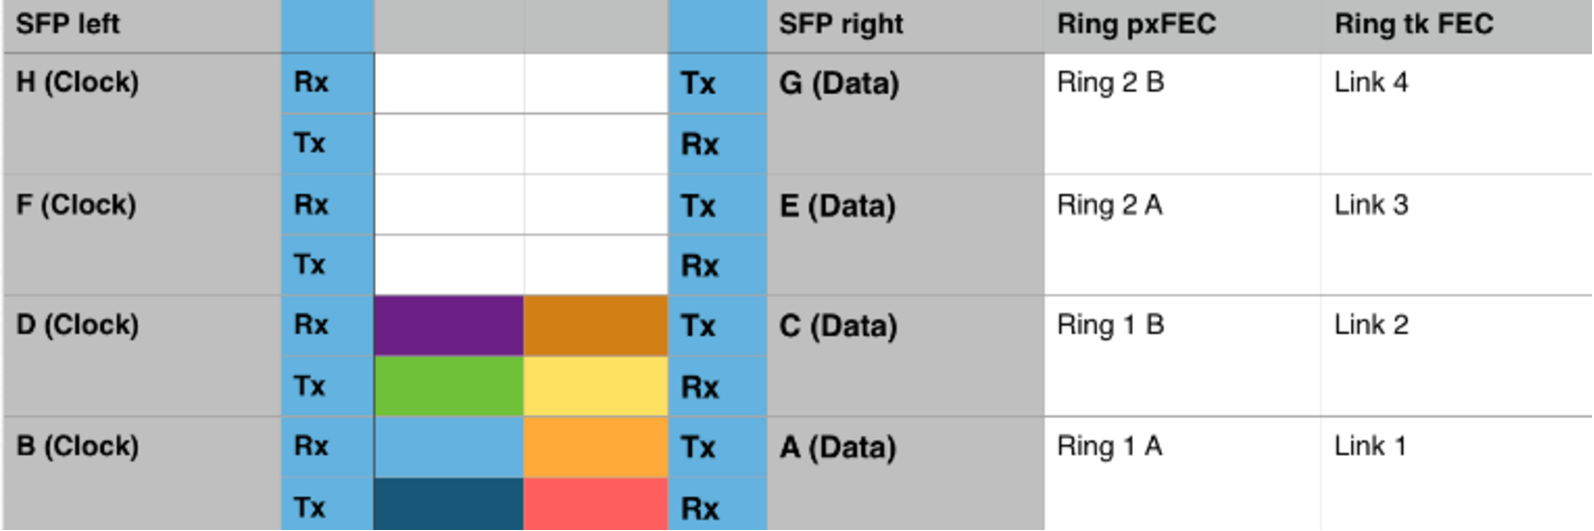
\includegraphics[width=\textwidth]{../images/FEC_fibre_mapping.pdf}
\caption[FEC fibre mapping]{\label{pic:FECFibreMapping} \textbf{FEC fibre mapping}\\
}
\end{figure}



% ******************************************************************************
\ifx\isEmbedded\undefined
\input{../biblio.tex}
\end{document}
\else
\fi
